% F087｜牛顿切线法快速求近似根｜05_traps.tex
% 继承上传模板的 LaTeX 环境；当前条目的内容独立编写。
\clearpage
\begin{trapbox}
\textbf{\textcolor{CTrap}{易错一：把零点误认为函数最低点}}
\par\medskip
\begin{center}
% F087｜tangent 原创简明教学示意图
\begin{tikzpicture}[>=stealth,scale=.82]
\draw[->] (0,0)--(7.6,0) node[right]{$x$};\draw[->] (.8,-1.4)--(.8,3.2) node[above]{$y$};
% 横向比例尺 x_point=8(x-2.65)，纵向比例尺 y_point=0.75(x^2-10)。
\draw[teal,thick,domain=2.76:3.48,samples=45] plot ({8*(\x-2.65)},{.75*(\x*\x-10)});
% 在真实点 x_0=3 的切线；交轴位置 x_1=19/6。
\draw[orange,thick] (2,-1.2)--(6,1.05);
\fill[orange] (2.8,-.75) circle (2pt) node[below left=5pt]{$x_0=3$};
\fill[orange] (4.1333,0) circle(2pt) node[below=7pt]{$x_1\approx3.1667$};
\node at (5.5,2.7){\small 用切线寻找新的交点};
\node[teal] at (5.7,1.9){\small $y=x^2-10$};
\end{tikzpicture}

\end{center}
\medskip
牛顿切线法一般寻找的是\textbf{$f(x)=0$ 的根}，不是自动寻找最低点。对 $f(x)=x^2-10$，正根是图像与横轴的交点，最低点却在 $x=0$。
\end{trapbox}
\clearpage
\begin{trapbox}
\textbf{\textcolor{CTrap}{易错二：忘记斜率不能为零}}
\par\medskip
\begin{center}
% F087｜square 原创简明教学示意图
\begin{tikzpicture}[>=stealth,scale=.9]
\node[draw,fill=teal!8,rounded corners,minimum width=7.3cm,minimum height=1.5cm,align=center] at (4,0) {$x_{n+1}=\dfrac12\left(x_n+\dfrac{A}{x_n}\right)$};
\node at (4,-1.2) {\small 正数 $x_n$ 与 $A/x_n$ 的平均数};
\end{tikzpicture}

\end{center}
\medskip
分母是 $f'(x_n)$，若为 $0$，公式不能直接使用。如对 $x^2-10$ 取 $x_0=0$，则除数为零；求正平方根应取正的初值。
\end{trapbox}
\clearpage
\begin{trapbox}
\textbf{\textcolor{CTrap}{易错三：把“迭代几次很准”理解为永远收敛}}
\par\medskip
\begin{center}
% F087｜steps 原创简明教学示意图
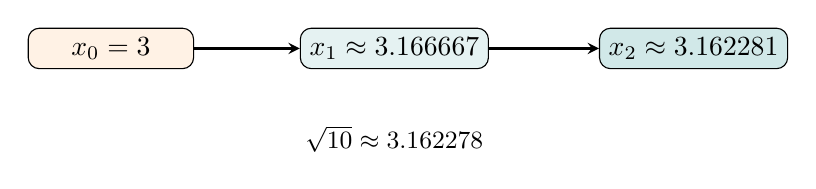
\begin{tikzpicture}[>=stealth,node distance=1cm]
\node[draw,rounded corners,fill=orange!10,minimum width=2.1cm] (a) at (0,0) {$x_0=3$};
\node[draw,rounded corners,fill=teal!10,minimum width=2.3cm] (b) at (3.6,0) {$x_1\approx3.166667$};
\node[draw,rounded corners,fill=teal!18,minimum width=2.3cm] (c) at (7.4,0) {$x_2\approx3.162281$};
\draw[->,thick] (a)--(b);\draw[->,thick] (b)--(c);
\node at (3.6,-1.15) {\small $\sqrt{10}\approx3.162278$};
\end{tikzpicture}

\end{center}
\medskip
任意方程或任意起点都可能失败；尤其初值离根太远、切线接近平行横轴时。算完必须代回检验。
\end{trapbox}
